% 
% ======================================================================
\RequirePackage{docswitch}
% \flag is set by the user, through the makefile:
%    make note
%    make apj
% etc.
\setjournal{\flag}

\documentclass[\docopts]{\docclass}

% You could also define the document class directly
%\documentclass[]{emulateapj}

% Custom commands from LSST DESC, see texmf/styles/lsstdesc_macros.sty
\usepackage{lsstdesc_macros}

\usepackage{graphicx}
\graphicspath{{./}{./figures/}}
\bibliographystyle{apj}

% Add your own macros here:



% 
% ======================================================================

\begin{document}

\title{ Inference of the Conditional Luminosity Function by Explicit Marginalization over All Individual Galaxy Parameters }

\maketitlepre

\begin{abstract}

We explore a hierarchical model for galaxy luminosities and halo masses whose hyperparameters govern the conditional luminosity function, and whose many individual object parameters are explicitly marginalized over. 
We investigate four techniques to perform the high dimensional marginalization, and comment on their performance.
Furthermore, we analyze how these techniques scale in different scenarios.

\end{abstract}

% Keywords are ignored in the LSST DESC Note style:
\dockeys{latex: templates, papers: awesome}

\maketitlepost

% ----------------------------------------------------------------------
%

\section{Introduction}
\label{sec:intro}

The large scale structure of the universe is dominated by the collective gravitational influence of dark matter particles and the repulsive force of dark energy. While there are ongoing efforts to infer the masses and locations of dark matter halos and improve measurements of dark energy parameters, observational progress has been gradual, encouraging alternative approaches. 
Hydrodynamic simulations have been an effective tool for bolstering our understanding of these contributors and their impact in structure formation and evolution.
Given a cosmology, large N-body simulations can predict characteristics like clustering and the halo mass function with high precision \citep*[eg.][]{nbody}. Virtual dark matter universes are readily available, and inspire us to explore ways to connect them to empirical observations.  

The halo mass and galaxy luminosity relation is one such conduit between dark matter halos and galaxy observations. 
The conditional probability allows us to convert the dark matter halos from simulations into distributions of galaxy luminosities in different redshift bins. 
These distributions can be compared to observed galaxy luminosities to further constrain the halos and relation. 
There has been work to determine the exact form of the relation and different models for centrals and satellite galaxies have been proposed \citep[eg.][]{satellites}.

Weak lensing is another technique that can characterize the halo composition of our universe. 
The gravitational influence of a massive dark matter halo causes the light from nearby galaxies to bend as it passes by, leading to a shearing effect. 
Over a swathe of sky, typically on the order of 1000 square arcminutes, the collective shears allow the masses and locations of halos to be weakly inferred. 
These inferences grow stronger as the density of galaxy observations increases.
The ongoing Dark Energy Survey and upcoming Large Synoptic Survey Telescope will provide dense galaxy catalogs which will benefit weak lensing \citep{des, lsst}. 

Traditionally the mass luminosity relation and weak lensing have been pursued in isolation, each ignoring information the other could provide. 
It is our goal to harness the full constraining power by modelling both weak lensing and the mass luminosity relation in a self consistent, heirarchical framework.
We employ the mass luminosity relation described in \citet{reddick} and the mass mapping infrastructure from 
\citet{components}. 
Figure \ref{fig:ultimate_pgm} outlines the dependencies of the model we aspire to build.

\begin{figure}[h]
\centering
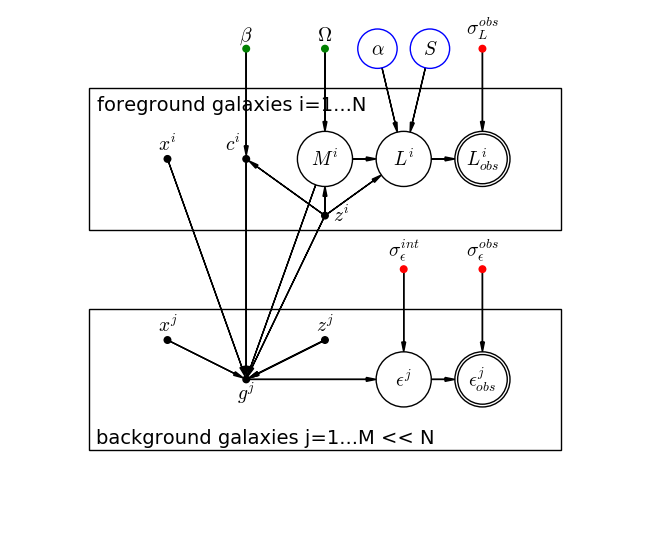
\includegraphics[width=0.9\columnwidth]{ultimate_pgm.png}
\caption{
A probabilistic graphical model for the model we ultimately aspire to. 
There are two plates; one for foreground galaxies, one for background galaxies. 
The cosmology hyperparameters are colored green, the mass luminosity relation hyperparameters are colored blue, and the noise hyperparameters are colored red. 
$\beta$ represents the form of the halo concentration.
$\Omega$ represents the cosmology used to generate the halos in the Millennium Simulation.
$\alpha$ represents four parameters that convert mass to mean luminosity, and $S$ represents the scatter of the corresponding lognormal.
$M,L$ represent mass and luminosity respectively. 
The variables $x,z$ denote angular position and redshift respectively.
$c$ is for the concentration, $g$ is for the reduced shear, and $\epsilon$ is for the shear.
Finally, $\sigma$ represents various forms of noise and the superscript \emph{obs} is used to denote an observational noise or observable. 
\label{fig:ultimate_pgm}}
\end{figure}

The model partitions galaxies into two groups. 
Background galaxies are sources that lie in a redshift bin immediately behind the three dimensional space of foreground galaxies. 
The background galaxies provide the observed shears which we use to infer the halo masses of foreground galaxies. 
We plan to use around 200,000 foreground galaxies and 1,600 background galaxies in our model and analysis. 
In the course of the heirarchical inference, each of the 200,000 galaxies contributes and has a corresponding mass and luminosity which must be marginalized out. 
Given the large size of our inference, we expect the primary challenges to be computational in nature - how can we achieve inference at this unprecedent scale?
In order for us to rapidly iterate towards an answer to this question, we study a model with simplified dependencies.
This condensed model, shown in Figure \ref{fig:simplified_pgm}, is easier to test and retains many of the computational challenges. 

\begin{figure}[h]
\centering
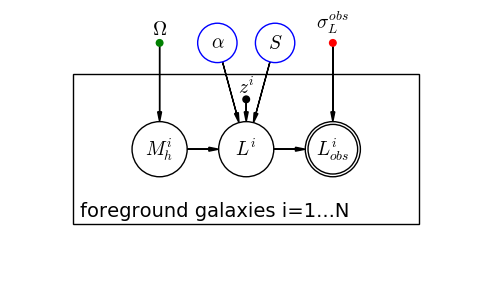
\includegraphics[width=0.9\columnwidth]{simplified_pgm.png}
\caption{
A probabilistic graphical model for the simplified model we will use for testing.
The parameters are a subset of those in Figure \ref{fig:ultimate_pgm}.
\label{fig:simplified_pgm}}
\end{figure}

The data we use ultimately comes from the Millennium Simulation \citep{millennium}. 
Our desire to eventually incorporate weak lensing components into our model drives our selection. 
\citet{raytracing} have performed raytracing which we plan to make use of in later analysis. 
A friend-of-friend (FoF) group finding algorithm identifies halos from particle concentrations. 
We carve out a $40 \times 40$ square arcminute window of sky out to redshift 3.5, and use the interior halos as the foreground galaxies in our analysis.  

The statistical inference we perform follows the canonical inference formula: posterior equals prior times likelihood. 
In the analysis that follows we use an overline, such as $\overline{z}$, to distinguish a vector over all foreground galaxies from the variable corresponding to a single halo, or $z$.
Given the mass luminosity hyperparameters $\alpha$, $S$; a vector of observed luminosities $\overline{L^{obs}}$; a vector of redshifts $\overline{z}$; and the observational noise in luminosity measurements $\sigma_L^{obs}$ - the posterior we seek is $P(\alpha, S| \overline{L^{obs}}, \overline{z}, \sigma_L^{obs}) = P(\alpha, S)P(\overline{L^{obs}}| \alpha, S, \overline{z}, \sigma_L^{obs})$. 
Using the probabilistic graphical model we factor this further to

\begin{align*}P(\alpha, S| \overline{L^{obs}}, \overline{z}, \sigma_L^{obs}) &= P(\alpha)P(S) \\
 \iint \overline{dM}\ \overline{dL}\ &P(\overline{L^{obs}}| L, \sigma_L^{obs}) P(\overline{L}|\overline{M},\alpha,S,\overline{z})P(\overline{M}|\overline{z})
\end{align*}

The likelihood integral involves integrating over 400,000 variables, the mass and luminosity for each galaxy in our dataset. 
The Methods section of this paper describes various approaches to make such a large integral computationally tractable. 

The integrand of the likelihood contains three probabilities. 
The first is the conditional observed luminosity probability. 
Since luminosities are usually reporeted in log-space, we assume that there are gaussian errors in the log-space luminosity measurements, or that the distribution is log-normal. 
We believe 5\% errors seem reasonable and fix $\sigma_L^{obs} = 0.05$. Our conditional distribution is 

$$P(\overline{L^{obs}}| \overline{L}, \sigma_L^{obs}) = \frac{1}{\overline{L^{obs}}\sigma_L^{obs}\sqrt{2\pi}}\exp\left(-\frac{(\ln \overline{L^{obs}} - \ln \overline{L})^2}{2\sigma_L^{obs\ 2}}\right)$$

The second factor in the likelihood integrand is the mass luminosity relation $P(\overline{L}|\overline{M},\alpha,S,\overline{z})$. 
We use the form described in (reddick's thesis). 
As in numerous previous studies, Reddick divides the conditional luminosity into two parts. 
The central galaxy is described by a lognormal distribution and the satellite galaxies are described by a Schechter function. 
In our analysis, we ignore the satellite contribution. 
This decision is made for convenience, and we can easily add the satellite contribution in future analyses. 
We use $\alpha = (\alpha_1, \alpha_2, \alpha_3, \alpha_4)$ to represent the parameters for computing the mean luminosity and $S$ for the scatter. 
This gives

\begin{align*}
P(\overline{L}|\overline{M},\alpha,S,\overline{z}) &= \frac{1}{\overline{L}S\sqrt{2\pi}}\exp\left(-\frac{(\ln \overline{L} - \ln \overline{\mu_L})^2}{2S^{2}}\right)\\
\mu_L &= \exp(\alpha_1) \cdot \left(\frac{M}{\alpha_3}\right)^{\alpha_2} \cdot (1+z)^{\alpha_4}\\
\end{align*}

The third factor in the likelihood integrand is the halo mass function $P(\overline{M}|\overline{z})$. 
For this we rely on the python software package hmfcalc \citep*{hmf}. 
We use the functional form from \citep{tinker} and the cosmology from the Millennium Simulation.


% ----------------------------------------------------------------------

\section{Methods}
\label{sec:methods}

\subsection{Test Dataset}
\label{subsec:testdata}

\subsection{Numerical Integration}
\label{subsec:numint}

\subsection{Simple Monte Carlo}
\label{subsec:smc}

\subsection{Importance Sampling}
\label{subsec:is}

Plots showing why biased distribution makes sense.

\subsection{Laplace Approximation}
\label{subsec:laplace}


% ----------------------------------------------------------------------

\section{Results}
\label{sec:results}

Compare single integrals.

Analyze how importance sampling and laplace approximation scale.


% ----------------------------------------------------------------------

\section{Discussion}
\label{sec:discussion}


Mention obvious tradeoffs between methods.

Mention BigMaLI codebase for repreoducibility.

Back of the envelope cluster scaling.

% ----------------------------------------------------------------------

\section{Conclusions}
\label{sec:conclusions}

Short summary.

% ----------------------------------------------------------------------

\subsection*{Acknowledgments}

Here is where you should add your specific acknowledgments, remembering that some standard thanks will be added via the \code{acknowledgments.tex} and \code{contributions.tex} files.

% 
This is the text imported from \code{acknowledgments.tex}, and will be replaced by some standard LSST DESC boilerplate at some point.
% 


\input{contributions}

%{\it Facilities:} \facility{LSST}

% Include both collaboration papers and external citations:
\bibliography{main}

\end{document}
% ======================================================================
% 
